\documentclass[conference]{IEEEtran}
\IEEEoverridecommandlockouts
% The preceding line is only needed to identify funding in the first footnote. If that is unneeded, please comment it out.
%Template version as of 6/27/2024

\usepackage{cite}
\usepackage{amsmath,amssymb,amsfonts}
\usepackage{algorithmic}
\usepackage{graphicx}
\usepackage{textcomp}
\usepackage{xcolor}
\usepackage{tikz}
\usepackage{physics}
\usepackage{algorithm}
\usepackage{pgfplots}
\usepackage{pgfplotstable}
\usepgfplotslibrary{statistics}
\usepackage{etoolbox} % for \ifnumcomp
\usepackage{listofitems} % for \readlist to create arrays
% \usepackage[ruled,vlined]{algorithm% Increase row height
\renewcommand{\arraystretch}{1.4}

% Adjust column spacing
\setlength{\tabcolsep}{8pt}  % default is 6pt, increasing it for better spacing

\tikzset{>=latex} % for LaTeX arrow head
\colorlet{myred}{red!80!black}
\colorlet{myblue}{blue!80!black}
\colorlet{mygreen}{green!60!black}
\colorlet{mydarkred}{myred!40!black}
\colorlet{mydarkblue}{myblue!40!black}
\colorlet{mydarkgreen}{mygreen!40!black}
\tikzstyle{node}=[very thick,circle,draw=myblue,minimum size=22,inner sep=0.5,outer sep=0.6]
\tikzstyle{connect}=[->,thick,mydarkblue,shorten >=1]
\tikzset{ % node styles, numbered for easy mapping with \nstyle
  node 1/.style={node,mydarkgreen,draw=mygreen,fill=mygreen!25},
  node 2/.style={node,mydarkblue,draw=myblue,fill=myblue!20},
  node 3/.style={node,mydarkred,draw=myred,fill=myred!20},
}
\def\nstyle{int(\lay<\Nnodlen?min(2,\lay):3)} % map layer number onto 1, 2, or 3

\usetikzlibrary{arrows.meta,shadows,positioning}
\usetikzlibrary{calc}
\usetikzlibrary{fit, positioning, shapes.geometric}
\tikzset{
	frame/.style={
		rectangle, draw,
		text width=6em, text centered,
		minimum height=4em,drop shadow,fill=white,
		rounded corners,
	},
	line/.style={
		draw, -{Latex},rounded corners=3mm,
	}
}
% Tikz Library
\usetikzlibrary{calc, quotes, angles}
\pgfmathsetmacro{\r}{0.8}	
\pgfmathsetmacro{\Phi}{-160}
\pgfmathsetmacro{\Theta}{-90}
\usepackage{fontawesome5}
\usepackage{float}
\def\BibTeX{{\rm B\kern-.05em{\sc i\kern-.025em b}\kern-.08em
    T\kern-.1667em\lower.7ex\hbox{E}\kern-.125emX}}
\begin{document}

\title{Robust DDPG Reinforcement Learning Differential Game Guidance in Low-Thrust, Multi-Body Dynamical Environments}
% *\\
% {\footnotesize \textsuperscript{*}Note: Sub-titles are not captured for https://ieeexplore.ieee.org  and
% should not be used}
% \thanks{Identify applicable funding agency here. If none, delete this.}
% }

\author{\IEEEauthorblockN{Hadi Nobahari}
\IEEEauthorblockA{\textit{Department of Aerospace Engineering} \\
\textit{Sharif University of Technology}\\
Tehran, Iran \\
nobahari@sharif.edu}
\and
\IEEEauthorblockN{Ali Baniasad}
\IEEEauthorblockA{\textit{Department of Aerospace Engineering} \\
\textit{Sharif University of Technology}\\
Tehran, Iran \\
ali\_baniasad@ae.sharif.edu}
}

\maketitle

\begin{abstract}
Onboard autonomy is a critical enabler for increasingly complex deep-space missions. In nonlinear dynamical environments, designing computationally efficient and robust guidance strategies remains a significant challenge. Traditional approaches often rely on simplifying assumptions in the dynamical model or require substantial computational resources, limiting their applicability for onboard implementation. This research introduces a robust reinforcement learning-based differential game approach to develop an adaptive closed-loop controller for low-thrust spacecraft guidance in multi-body dynamical environments. The proposed controller is trained to handle large initial deviations, enhance resilience against disturbances, and augment conventional targeting guidance methods. Unlike traditional approaches, it does not require explicit knowledge of the dynamical model, allowing direct interaction with the nonlinear equations of motion to create a generalizable learning framework. High-performance computing is leveraged to train a robust neural network controller, which can be deployed onboard to generate real-time low-thrust control profiles without overloading the flight computer. The effectiveness of this method is demonstrated through sample transfers between Lyapunov orbits in the Earth-Moon system, where the controller exhibits strong robustness to perturbations and generalizes effectively across different mission scenarios and low-thrust engine models. This work highlights the potential of reinforcement learning-based differential game approaches in advancing autonomous spacecraft navigation in complex gravitational environments.
\end{abstract}

\begin{IEEEkeywords}
component, formatting, style, styling, insert.
\end{IEEEkeywords}

\section{Introduction}
\section{Problem Formulation}
The three-body problem provides a representative dynamical model for natural motion in cislunar space. Although the proposed guidance framework is not dependent on a specific dynamical model, the planar Circular Restricted Three-Body Problem (CR3BP) is employed as a test environment for preliminary evaluation. The CR3BP presents a complex yet relevant dynamical setting for upcoming space missions while maintaining a sufficiently low-fidelity structure for an initial assessment of the guidance scheme. Furthermore, low-thrust propulsion is incorporated to evaluate the algorithm's performance under conditions of limited control authority and significant nonlinearities. While the proposed guidance scheme directly generates a control history, an alternative operational approach involves utilizing the trained neural network to provide an initial guess for numerical methods such as targeting or optimization techniques. To illustrate this approach, a direct multiple shooting algorithm is included in the analysis, demonstrating the neural network's contribution to onboard targeting capabilities.
\subsection{Dynamical Model}
The Circular Restricted Three-Body Problem (CR3BP) models the motion of an infinitesimal mass under the gravitational influence of two primary celestial bodies. In this framework, two spherically symmetric masses, Earth and Moon, constitute the primary system, orbiting their common barycenter in circular trajectories. The third body, spacecraft, moves freely with respect to the barycenter, as illustrated in Fig.~\ref{fig:CR3BP}. The relative size of the primaries is characterized by the mass ratio  
\begin{equation}
	\mu = \frac{M_2}{M_1 + M_2},
\end{equation}
where \( M_1 \) is Earth mass and \( M_2 \) is Moon mass.	
Furthermore, the model assumes that the mass of the spacecraft is negligible compared to those of the primary bodies, thereby exerting no influence on their motion. The state of the spacecraft, defined by its position and velocity vectors \( \vb{r}\) and \( \vb{v}\), respectively, is represented as  
\begin{equation}
	\boldsymbol{\rho}_{\text{spatial}} = \begin{bmatrix} x & y & z & \dot{x} & \dot{y} & \dot{z} \end{bmatrix}^T.
\end{equation}

These state components are propagated with respect to the barycenter in a rotating reference frame, depicted by dashed lines in Fig.~\ref{fig:CR3BP}.
\begin{figure}[H]
	\centering
    \resizebox{\linewidth}{!}{ 
	\begin{tikzpicture}
		% Coordinates
		\coordinate (earth) at (1,2);
		\coordinate (moon) at (8,1);
		\coordinate (earth-point1) at ({\r*cos(\Theta)+1},{\r*sin(\Theta)+2});
		\coordinate (A) at (-.5,.5);
		\coordinate (B) at (8.5,-0.5);
		
		% Earth
		\draw[thick, fill=black!30, draw=black!30
		] (earth) circle (\r);
		% Text
		\node (a) at (A) {Earth};
		
		% Moon
		\node[circle, inner sep=5.5pt, fill=black!30] (MOON) at (moon) {};
		% Text 
		\node[below, shift={(0,-0.4)}] at (MOON) {$m$};
		\node (b) at (B) {Moon};
		
		% Lines
		% \draw[-latex] (earth) -- (MOON) node[pos=.55, below left] {$\vb{r}_o$};
		% \draw[-latex] (earth) -- (earth-point1) node [pos=0.6, left] {$\vb{r}$};
		\draw[-stealth] (a) to[bend left=30] ({\r*cos(\Phi)+1},{\r*sin(\Phi)+2});
		\draw[-stealth] (b) to[bend left=-30] (MOON);
		\draw[dashed, black] (earth) -- (MOON.center);
		
		% center of mass 0.25 from earth
		\coordinate (center) at ($(earth)!0.3!(MOON)$);
		% small circle
		\draw[fill=black] (center) circle (1.5pt) node[below, shift={(0,-0.1)}] {Barycenter};
		% add satellite with shift
		\coordinate (satellite) at ($(center)!0.5!(MOON)+(0,2)$);
		% \node at ($(center)!0.5!(MOON)+(0,2)$) {\faSatellite};
		% shift coordinate
		\node (satellite) at (satellite) {\faSatellite};
		
		% connect earth to satellite r1
		\draw[-stealth] (earth) -- (satellite) node[pos=0.75, above] {$\vb{r}_1$};   
		% connect moon to satellite r2
		\draw[-stealth] (MOON) -- (satellite) node[pos=0.5, above] {$\vb{r}_2$};
		% connect center of mass to satellite r
		\draw[-stealth] (center) -- (satellite) node[pos=0.5, above] {$\vb{r}$};
		% add line to show satellite is in between
		\node (c) at ($(satellite)+(1.5,0.5)$) {Spacecraft};
		\draw[-stealth] (c) to[bend left=30] (satellite);
		% add x y axis from center of mass connect to moon
		\draw[-stealth] (center) -- ($(center)!0.5!(MOON)$) node[below] {$\hat x$};
		% plot y vertical to x
		\draw[-stealth] (center) -- ($(center)+(0.4,2)$) node[left] {$\hat y$};
	\end{tikzpicture}}
	\caption{Planar CR3BP vector definitions}\label{fig:CR3BP}
\end{figure}


Many mission architectures benefit from the integration of low-thrust electric propulsion systems. Unlike traditional chemical propulsion engines, electric propulsion systems offer significantly higher efficiency; however, they are characterized by delivering energy changes over extended time periods. One prominent type of low-thrust engine employed in Solar Electric Propulsion (SEP) systems is the ion thruster, which is powered by solar panels mounted on the spacecraft. Ion thrusters have been successfully utilized in a number of space missions, such as NASA's \textit{Deep Space 1} \cite{DeepSpace1} and \textit{Dawn} \cite{Dawn}, among others. Building upon this successful application, future low-thrust missions include \textit{Psyche} \cite{Psyche} and the \textit{Lunar Gateway} \cite{LunarGateway}. The present study assumes that spacecraft is equipped with a Constant Specific Impulse (CSI) low-thrust engine. The additional propulsion force provided by this engine modifies the natural equations of motion in the Circular Restricted Three-Body Problem (CR3BP), introducing low-thrust terms to the governing equations.

\begin{align}
	% \begin{split}
		\ddot{x} &= 2\dot{y} + x - \frac{(1-\mu)(x+\mu)}{r_1^3} - \frac{\mu(x-1+\mu)}{r_2^3} + u_x, \\
		\ddot{y} &= -2\dot{x} + y - \frac{(1-\mu)y}{r_1^3} - \frac{\mu y}{r_2^3} + u_y, \\
		\ddot{z} &= -\frac{(1-\mu)z}{r_1^3} - \frac{\mu z}{r_2^3} + u_z,
	% \end{split}
\end{align}
where the control inputs \( u_x \), \( u_y \), and \( u_z \) represent the thrust components along the spacecraft's body-fixed axes. The distances \( r_1 \) and \( r_2 \) are defined as 
\begin{align}
	r_1 &= \sqrt{(x+\mu)^2 + y^2 + z^2}, \\
	r_2 &= \sqrt{(x-1+\mu)^2 + y^2 + z^2}.
\end{align}
The state-space representation of the CR3BP with low-thrust terms is given by
\begin{equation}
	\dot{\boldsymbol{\rho}} = \boldsymbol{f}(\boldsymbol{\rho}, \boldsymbol{u}),
\end{equation}
where \( \boldsymbol{\rho} \) is the state vector and \( \boldsymbol{u} \) is the control input vector. The state-space representation is used to define the spacecraft's trajectory in the CR3BP, incorporating the effects of the low-thrust engine.


\subsection{Low-Thrust Control Problem}
The motion in the Circular Restricted Three-Body Problem (CR3BP) is inherently nonlinear, displaying notably sensitive dynamical structures. Consequently, the proposed guidance strategy capitalizes on the influence of the low-thrust terms to achieve the desired dynamical behavior. As elaborated by Cox et al. \cite{Cox201X}, the thrust direction is determined by the low-thrust acceleration vector, defined as:
\begin{equation}
\mathbf{a}_{lt} = a_{lt} \hat{u}_x \hat{i} + a_{lt} \hat{u}_y \hat{j} + a_{lt} \hat{u}_z \hat{k},
\end{equation}
where \( \hat{u}_x \), \( \hat{u}_y \), and \( \hat{u}_z \) are the components of the thrust unit vector in the rotating frame of the CR3BP, and \( a_{lt} \) represents the low-thrust acceleration components in the corresponding directions. Furthermore, the thrust direction is characterized by the thrust magnitude \( f \) and the spacecraft's nondimensional mass \( m = \frac{M_3}{M_{3,0}} \), where \( M_3 \) denotes the spacecraft mass at the beginning of the thrust segment and \( M_{3,0} \) is the initial mass.

The thrust direction is oriented by the unit vector \( \hat{u} \), which remains fixed in the rotating frame of the CR3BP during each integration step. While it may be impractical to consider a continuously changing inertial thrust direction, the current study focuses on thrust segments of 20.87 hours. The precession of the rotating frame during these intervals can be addressed when transitioning the CR3BP solutions into a higher-fidelity model. It is also important to note that propulsive capability is inversely related to the spacecraft's mass, such that as propellant is consumed, the spacecraft gains a higher thrust-to-mass ratio. 

The nondimensional thrust magnitude \( f \) is computed as follows:
\begin{equation}
f = \frac{l^* M_{3,0}}{F_t^*},
\end{equation}
where \( F_t^* \) is the thrust in kilonewtons, and \( M_{3,0} \) is the initial mass of the spacecraft in kilograms. For the purposes of this investigation, a sample spacecraft is considered, which has a maximum propulsive capability of \( f_{\text{max}} = 0.04 \). A comparison between this sample spacecraft and other previous and planned engine capabilities is summarized in Table \ref{tab:comparison}. The sample spacecraft exhibits a propulsive capability comparable to that of the planned Psyche spacecraft, which exceeds that of Hayabusa 1, Hayabusa 2, Dawn, and Lunar IceCube, but is less than the capabilities of Deep Space 1. As a nondimensional quantity, this thrust level can represent any spacecraft with the same thrust-to-mass ratio. Specifically, \( f_{\text{max}} = 0.04 \) models an 11.46 kg spacecraft equipped with a BIT-3 CubeSat engine \cite{LunarIceCube} (intended for use on Lunar IceCube and LunaH-Map) as well as an 850.2 kg spacecraft utilizing an NSTAR engine \cite{DeepSpace1} (employed on Deep Space 1 and Dawn).
\begin{table*}[h!]
	\centering
	\caption{Low-thrust capability of various spacecraft, nondimensionalized in the Earth-Moon system.}
	\begin{tabular}{|l|l|l|l|l|}
	\hline
	\textbf{Abbrv.} & \textbf{Spacecraft} & \textbf{$f_{\text{max, nondim}}$} & \textbf{$M_{3,0}$ (kg)} & \textbf{$F_{\text{max}}$ (mN)} \\ \hline
	H1 & Hayabusa 1 \cite{40} & $1.640 \cdot 10^{-2}$ & 510 & 22.8 \\ \hline
	H2 & Hayabusa 2 \cite{41} & $1.628 \cdot 10^{-2}$ & 608.6 & 27.0 \\ \hline
	LIC & Lunar IceCube \cite{3,39} & $3.276 \cdot 10^{-2}$ & 14 & 1.25 \\ \hline
	Dawn & Dawn \cite{37} & $2.741 \cdot 10^{-2}$ & 1217.8 & 91.0 \\ \hline
	DS1 & Deep Space 1 \cite{36} & $6.940 \cdot 10^{-2}$ & 486.3 & 92.0 \\ \hline
	Psyche & Psyche \cite{5,42} & $4.158 \cdot 10^{-2}$ & 2464 & 279.3 \\ \hline
	s/c & Sample spacecraft & $4 \cdot 10^{-2}$ & n/a & n/a \\ \hline
	\end{tabular}
	\label{tab:camparison}	
\end{table*}
	




\section{Guidance Framework Design}
The proposed guidance framework leverages reinforcement learning to develop a robust differential game-based guidance strategy for low-thrust spacecraft in multi-body dynamical environments. The guidance strategy is designed to handle large initial deviations, enhance resilience against disturbances, and augment conventional targeting guidance methods. The framework is implemented using the Deep Deterministic Policy Gradient (DDPG) algorithm, which is a model-free, off-policy reinforcement learning algorithm that combines the stability of deterministic policy gradients with the flexibility of deep neural networks. The DDPG algorithm is well-suited for continuous action spaces and has been successfully applied to a variety of control problems, including robotic manipulation and locomotion tasks. The guidance strategy is trained using a differential game formulation, where two spacecraft are modeled as agents in a competitive game. The agents interact with each other and the environment to learn optimal control policies that maximize their rewards. The guidance strategy is implemented in a simulated environment that captures the dynamics of the Circular Restricted Three-Body Problem (CR3BP) with low-thrust terms. The effectiveness of the guidance strategy is demonstrated through sample transfers between Lyapunov orbits in the Earth-Moon system, where the controller exhibits strong robustness to perturbations and generalizes effectively across different mission scenarios and low-thrust engine models. The proposed guidance framework represents a significant advancement in autonomous spacecraft navigation in complex gravitational environments and has the potential to enable a wide range of deep-space missions.
\subsection{Reinforcement Learning Overview}
Reinforcement learning is a machine learning paradigm that enables agents to learn optimal control policies by interacting with an environment to maximize cumulative rewards. The agent observes the state of the environment, selects actions based on its policy, receives rewards from the environment, and updates its policy to improve its performance over time. The goal of the agent is to learn an optimal policy that maximizes its expected cumulative reward.
\subsubsection{Neural Networks}
Neural networks are a class of machine learning models that are inspired by the structure and function of the human brain. They consist of interconnected nodes, or neurons, organized in layers. Each neuron takes input from the previous layer, applies a nonlinear activation function, and produces an output that is passed to the next layer. Neural networks are capable of learning complex patterns and relationships in data and have been successfully applied to a wide range of machine learning tasks, including image recognition, natural language processing, and reinforcement learning.
\subsubsection{Reinforcement Learning Fundamentals}
Reinforcement learning (RL) refers to a class of algorithms wherein a goal-directed agent seeks to accomplish a task through interaction with an environment. An agent is defined as a controller that maps observed variables (states) to corresponding actions. The learning process initiates with the agent exploring the environment through trial-and-error. The environment conveys relevant information about its dynamics to the agent in the form of a state signal, which the agent utilizes to determine an appropriate action. In response to the action, the environment updates its state and computes a numerical reward, representing the immediate benefit derived from the action taken. This iterative process continues, enabling the agent to refine its policy—the strategy it employs to make decisions—with the objective of maximizing the reward signal over time.

In many RL scenarios, terminal conditions are introduced, resulting in the cessation of the learning process. In such cases, the environment typically resets to an initial configuration, and the learning process recommences. These situations are classified as episodic tasks, where each episode represents a discrete attempt by the agent to solve a problem. A high-level schematic of the RL process is presented in Fig. 3. This diagram illustrates the three key signals—state, action, and reward—that facilitate communication between the agent and the environment at discrete time steps, \( t \) and \( t+1 \). While the RL literature predominantly uses the terminology of agent, environment, and action, these terms are conceptually analogous to the more commonly used engineering terminology of controller, controlled system (or plant), and control signal \cite{48}.
\begin{figure}[H]
	\begin{center}
	\resizebox{\linewidth}{!}{ 
	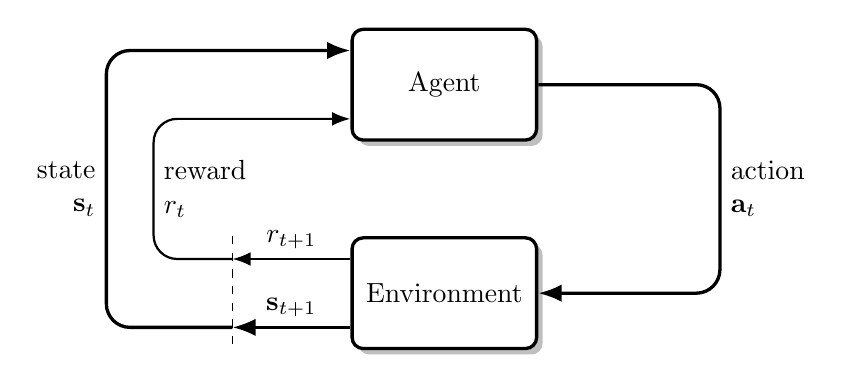
\begin{tikzpicture}[very thick,node distance = 4cm]
			\node [frame] (agent) {Agent};
			\node [frame, below=1.2cm of agent] (environment) {Environment};
			\draw[line] (agent) -- ++ (3.5,0) |- (environment) 
			node[right,pos=0.25,align=left] {action\\ $\vb{a}_t$};
			\coordinate[left=15mm of environment] (P);
			\draw[thin,dashed] (P|-environment.north) -- (P|-environment.south);
			\draw[line] (environment.200) -- (P |- environment.200)
			node[midway,above]{$\vb{s}_{t+1}$};
			\draw[line,thick] (environment.160) -- (P |- environment.160)
			node[midway,above]{$r_{t+1}$};
			\draw[line] (P |- environment.200) -- ++ (-1.6,0) |- (agent.160)
			node[left, pos=0.25, align=right] {state\\ $\vb{s}_t$};
			\draw[line,thick] (P |- environment.160) -- ++ (-1,0) |- (agent.200)
			node[right,pos=0.25,align=left] {reward\\ $r_t$};
		\end{tikzpicture}}
	\end{center}
	\caption{The agent-environment process in a Markov decision process \cite{Sutton}.}
	\label{fig:agent_env}
\end{figure}

Without external supervision, the agent uncovers complex dynamical structures that inform its decision-making. This process is characterized as a Markov Decision Process (MDP), which incorporates both feedback and associative actions, representing a classical formalization of sequential decision-making problems \cite{48}. The MDP serves as the idealized mathematical framework for the problem, enabling theoretical analysis of the reinforcement learning (RL) process. In the infinite-horizon discounted case, the MDP is formulated as a tuple \( \langle S, A, P, r, q_0, \gamma \rangle \), where \( S \) and \( A \) denote the sets of all possible states and actions, respectively; \( P : S \times A \times S \to [0, 1] \) represents the state-transition probability distribution; \( r : S \to \mathbb{R} \) is the reward function; \( q_0 \) is the distribution of the initial states \( s_0 \); and \( \gamma \in [0, 1] \) is the discount factor \cite{49}.

For a problem to be accurately cast as an MDP, it must satisfy the Markov property, which asserts that future states depend solely on the current state, and not on the sequence of prior events \cite{48}. In many practical applications, only partial information is available, and the agent is provided with a subset of the total environmental data. This partial information is referred to as the "observation," which serves as an analog to the state signal. Such systems, characterized by reduced information, are classified as Partially Observable Markov Decision Processes (POMDPs). The distinction between state and observation is crucial in POMDPs, as it emphasizes the fact that the agent operates based on incomplete information. However, this investigation assumes a fully observable MDP, and for the sake of simplicity, the observation \( o_t \) is treated as the state \( s_t \), rendering the distinction unnecessary.

An agent seeks to develop a policy that maximizes its expected future reward by balancing immediate and future returns. This balance is formalized by defining the expected return \( G_t \) as the sum of future discounted rewards, expressed as:
\begin{align}
    G_t =& r_{t+1} + \gamma r_{t+2} + \gamma^2 r_{t+3} + \cdots + \gamma^{T-t-1} r_T \\=& \sum_{k=t+1}^{T} \gamma^{k-t-1} r_k,
\end{align}
where \( \gamma \in [0, 1] \) is the discount factor that determines the relative importance of immediate versus future rewards. When \( \gamma = 1 \), all future rewards are considered equally important; when \( \gamma = 0 \), only the immediate reward is taken into account. The definition of expected return leads to the formalization of the value function, which is estimated in nearly all RL algorithms and informs the agent of the quality of a particular state. For an MDP, the state-value function \( V^\pi(s_t) \) is defined as
\begin{equation}
	V^\pi(s_t) = \mathbb{E}_\pi \left[ G_t | s_t \right] = \mathbb{E}_\pi \left[ \sum_{k=t+1}^{T} \gamma^{k-t-1} r_k | s_t \right],
\end{equation}	
where \( \pi \) denotes the policy that the agent follows. The action-value function \( Q^\pi(s_t, a_t) \) is defined as
\begin{equation}
	Q^\pi(s_t, a_t) = \mathbb{E}_\pi \left[ G_t | s_t, a_t \right] = \mathbb{E}_\pi \left[ \sum_{k=t+1}^{T} \gamma^{k-t-1} r_k | s_t, a_t \right],
\end{equation}
which represents the expected return when the agent is in state \( s_t \), takes action \( a_t \), and follows policy \( \pi \) thereafter. The value functions and action-value functions are related by
\begin{equation}
	V^\pi(s_t) = \mathbb{E}_{a_t \sim \pi} \left[ Q^\pi(s_t, a_t) \right].
\end{equation}
Policy optimization methods aim to directly learn a parameterized policy, \( \pi_\theta(a | s) \), where \( \theta \) represents the policy parameter vector. Unlike value optimization methods, such as \( Q \)-Learning and Deep Q-Networks (DQN), policy optimization methods are particularly well-suited for problems involving continuous action spaces. The ability to incorporate both continuous state and action spaces provides a significant advantage in complex control tasks, where discretization can be a limitation, and also enhances the extendibility to higher-dimensional dynamical models.

A notable subset of reinforcement learning (RL) methods arises from hybrid algorithms, commonly known as actor-critic methods. These approaches concurrently learn the policy (i.e., the actor) and the value function (i.e., the critic), where both the actor and the critic are often represented as neural networks. Among the various actor–critic schemes, Deep Deterministic Policy Gradient (DDPG) \cite{52} is particularly relevant for continuous action spaces and is employed in this investigation. DDPG has shown significant success in high-dimensional continuous control tasks and is the method of choice for this study.


\subsubsection{Deep Deterministic Policy Gradient}
\section{Deep Deterministic Policy Gradient (DDPG)}

Deep Deterministic Policy Gradient (DDPG) is an off-policy, model-free, and actor-critic reinforcement learning algorithm that is particularly well-suited for problems involving continuous action spaces. It is an extension of the Deterministic Policy Gradient (DPG) algorithm, incorporating deep neural networks to approximate both the policy and value functions. DDPG is based on the idea that the policy can be directly optimized by learning a deterministic policy function, and the value function can be approximated using the Q-function. Below, we describe the key components and the mathematical formulation of DDPG.

\subsection{Policy and Value Functions}

In DDPG, the agent learns a deterministic policy \( \pi_{\theta}(s) \), which maps states \( s \) directly to actions \( a \). The policy is parameterized by a neural network with weights \( \theta \), and the goal is to find the policy that maximizes the expected return.

The action-value function (Q-function) is defined as the expected return of taking action \( a \) in state \( s \), following the policy \( \pi \). The Q-function is given by:

\begin{equation}
    Q^{\pi}(s, a) = \mathbb{E} \left[ \sum_{t=0}^{T} \gamma^t r_t | s_0 = s, a_0 = a, \pi \right],
\end{equation}
where \( r_t \) denotes the reward received at time step \( t \), and \( \gamma \in [0, 1] \) is the discount factor. The goal of DDPG is to learn the optimal action-value function, \( Q^{\pi^*}(s, a) \), which provides the expected return for each state-action pair under the optimal policy.

\subsection{DDPG Objective}

The DDPG algorithm involves optimizing two primary functions: the policy function (actor) and the Q-function (critic). The actor is responsible for selecting actions, while the critic evaluates these actions by computing the Q-value.

The policy gradient is given by the deterministic policy gradient theorem, which states that the gradient of the expected return with respect to the policy parameters can be expressed as:

\begin{equation}
    \nabla_{\theta} J(\theta) = \mathbb{E} \left[ \nabla_{\theta} \pi_{\theta}(s) \nabla_a Q(s, a) |_{a = \pi_{\theta}(s)} \right],
\end{equation}
where \( \nabla_{\theta} \pi_{\theta}(s) \) is the gradient of the policy with respect to its parameters, and \( \nabla_a Q(s, a) \) is the gradient of the Q-function with respect to the action.

For the Q-function, the update rule is based on the Bellman equation for continuous action spaces, which provides a target for the Q-function update. The Bellman backup equation is given by:

\begin{equation}
    y = r + \gamma Q'(s', a'; \theta^-),
\end{equation}
where \( r \) is the immediate reward, \( s' \) is the next state, \( a' \) is the action chosen by the target policy \( \pi_{\theta^-}(s') \), and \( Q'(s', a'; \theta^-) \) is the target Q-value. The target Q-value is estimated using the target Q-network, which has parameters \( \theta^- \) and is periodically updated to stabilize training.

\subsection{DDPG Algorithm}

The DDPG algorithm is implemented using two neural networks: the actor network \( \pi_{\theta}(s) \) and the critic network \( Q_{\theta}(s, a) \). These networks are trained using the following algorithm:

\begin{algorithm}[H]
    \caption{Deep Deterministic Policy Gradient}
    \label{alg1}
\begin{algorithmic}[1]
    \STATE Input: initial policy parameters $\theta$, Q-function parameters $\phi$, empty replay buffer $\mathcal{D}$
    \STATE Set target parameters equal to main parameters $\theta_{\text{targ}} \leftarrow \theta$, $\phi_{\text{targ}} \leftarrow \phi$
    \REPEAT
        \STATE Observe state $s$ and select action $a = \text{clip}(\mu_{\theta}(s) + \epsilon, a_{Low}, a_{High})$, where $\epsilon \sim \mathcal{N}$
        \STATE Execute $a$ in the environment
        \STATE Observe next state $s'$, reward $r$, and done signal $d$ to indicate whether $s'$ is terminal
        \STATE Store $(s,a,r,s',d)$ in replay buffer $\mathcal{D}$
        \STATE If $s'$ is terminal, reset environment state.
        \IF{it's time to update}
            \FOR{however many updates}
                \STATE Randomly sample a batch of transitions, $B = \{ (s,a,r,s',d) \}$ from $\mathcal{D}$
                \STATE Compute targets
                \begin{equation*}
                    y(r,s',d) = r + \gamma (1-d) Q_{\phi_{\text{targ}}}(s', \mu_{\theta_{\text{targ}}}(s'))
                \end{equation*}
                \STATE Update Q-function by one step of gradient descent using
                \begin{equation*}
                    \nabla_{\phi} \frac{1}{|B|}\sum_{(s,a,r,s',d) \in B} \left( Q_{\phi}(s,a) - y(r,s',d) \right)^2
                \end{equation*}
                \STATE Update policy by one step of gradient ascent using
                \begin{equation*}
                    \nabla_{\theta} \frac{1}{|B|}\sum_{s \in B}Q_{\phi}(s, \mu_{\theta}(s))
                \end{equation*}
                \STATE Update target networks with
                \begin{align*}
                    \phi_{\text{targ}} &\leftarrow \rho \phi_{\text{targ}} + (1-\rho) \phi \\
                    \theta_{\text{targ}} &\leftarrow \rho \theta_{\text{targ}} + (1-\rho) \theta
                \end{align*}
            \ENDFOR
        \ENDIF
    \UNTIL{convergence}
\end{algorithmic}
\end{algorithm}


\subsection{Exploration and Exploitation}
In DDPG, the exploration of the environment is achieved by adding noise to the action selection process. This noise, typically Gaussian or Ornstein-Uhlenbeck noise, encourages the agent to explore the environment while still utilizing the learned policy. The balance between exploration and exploitation is maintained throughout the training process, with the noise gradually decaying as the policy converges.




\subsubsection{Differential Game Formulation}
In the context of zero-sum games, the differential game formulation provides a mathematical framework for modeling dynamic strategic interactions between two competing players. In such games, one player's gain is exactly the other player's loss, making it a zero-sum game. The formulation is typically used in control theory and reinforcement learning to model competitive scenarios where the players continuously adjust their strategies over time, based on the state of the game and the actions of their opponents.

Consider a scenario where two players, denoted as Player 1 and Player 2, interact over time, and each player aims to optimize their respective performance based on their actions. The game is defined over a continuous time interval, and the state of the system evolves according to differential equations that are influenced by the players' control inputs. Let the state of the system at time \( t \) be denoted by \( x(t) \), and the control inputs (actions) of Player 1 and Player 2 at time \( t \) be represented by \( u_1(t) \) and \( u_2(t) \), respectively.

The state dynamics of the system can be described by the following differential equations:
\begin{equation}
    \dot{x}(t) = f(x(t), u_1(t), u_2(t)),
\end{equation}
where \( f(x(t), u_1(t), u_2(t)) \) is a function that defines the system's evolution based on the current state \( x(t) \) and the control inputs \( u_1(t) \) and \( u_2(t) \).

Each player seeks to minimize (or maximize) a cost functional, depending on the game. The objective for Player 1 is to minimize the following cost function:
\begin{equation}
    J_1 = \int_{0}^{T} L_1(x(t), u_1(t), u_2(t)) dt + \Phi_1(x(T)),
\end{equation}
where \( L_1(x(t), u_1(t), u_2(t)) \) is the running cost for Player 1, and \( \Phi_1(x(T)) \) is the terminal cost at the end of the time horizon \( T \). Similarly, Player 2 seeks to minimize their own cost functional:
\begin{equation}
    J_2 = \int_{0}^{T} L_2(x(t), u_1(t), u_2(t)) dt + \Phi_2(x(T)),
\end{equation}
where \( L_2(x(t), u_1(t), u_2(t)) \) and \( \Phi_2(x(T)) \) represent the running and terminal costs for Player 2, respectively.

Given that this is a zero-sum game, the cost function for Player 1 is the negative of Player 2's cost, i.e., \( J_1 = -J_2 \). Therefore, the objective of each player is to optimize their own strategy while considering the opponent's strategy, leading to a competitive interaction between the two players.

The solution to the differential game involves determining the optimal control inputs \( u_1^*(t) \) and \( u_2^*(t) \) for Player 1 and Player 2, respectively. These are typically found by solving the Hamilton-Jacobi-Bellman (HJB) equations or by using the Pontryagin's Maximum Principle (PMP). The HJB equations for Player 1 and Player 2 are derived by first constructing the Hamiltonian functions for each player:

\begin{equation}
    H_1 = L_1(x(t), u_1(t), u_2(t)) + \lambda(t) \cdot f(x(t), u_1(t), u_2(t)),
\end{equation}
for Player 1, and
\begin{equation}
    H_2 = L_2(x(t), u_1(t), u_2(t)) + \mu(t) \cdot f(x(t), u_1(t), u_2(t)),
\end{equation}
for Player 2, where \( \lambda(t) \) and \( \mu(t) \) are the co-state variables associated with the state dynamics. The optimal strategies for both players are determined by solving these equations, subject to the appropriate boundary conditions and constraints.

The differential game formulation for a zero-sum game captures the dynamic nature of the competition between two players, where each player's objective is to minimize their own cost while simultaneously considering the opponent's strategy. The solution involves solving optimal control problems that account for both the state dynamics and the interaction between the players, providing insights into the optimal strategies for competitive environments.

\subsection{Environment Configuration}
The environment for the differential game-based guidance strategy is designed to capture the dynamics of the Circular Restricted Three-Body Problem (CR3BP) with low-thrust terms. The CR3BP is a classical dynamical system that models the motion of a spacecraft in the vicinity of two primary bodies, such as the Earth and the Moon, where the gravitational forces of the two bodies dominate the spacecraft's motion. The low-thrust terms represent the effects of a continuous thrust engine on the spacecraft's trajectory, allowing for more precise control over the spacecraft's motion.
\subsubsection{State Representation}
The state of the environment is defined by the position and velocity vectors of the spacecraft in the rotating frame of the CR3BP. The state vector is given by \( \boldsymbol{s} = \begin{bmatrix}
	\delta x & \delta y & \delta \dot{x} & \delta \dot{y}
\end{bmatrix}^\mathrm{T} \), where \( \delta x \) and \( \delta y \) are the deviations in the spacecraft's position from the nominal trajectory, and \( \delta \dot{x} \) and \( \delta \dot{y} \) are the deviations in the spacecraft's velocity. The state vector captures the relative position and velocity of the spacecraft with respect to the nominal trajectory, providing the necessary information for the guidance strategy to make decisions.
\subsubsection{Action Representation}
The action space of the environment corresponds to the control inputs of the spacecraft, which are the thrust components along the spacecraft's body-fixed axes. The action vector is given by \( \boldsymbol{a} = \begin{bmatrix}
	u_x & u_y
\end{bmatrix}^\mathrm{T} \), where \( u_x \) and \( u_y \) represent the thrust components along the spacecraft's body-fixed axes. The action space allows the guidance strategy to adjust the thrust direction and magnitude to control the spacecraft's trajectory.
\subsubsection{Reward Function}
The reward function of the environment is designed to incentivize the spacecraft to reach the desired Lyapunov orbit while minimizing deviations from the nominal trajectory. The reward function is defined as:
\begin{equation}
	r = -\alpha \left( \delta x^2 + \delta y^2 \right) - \beta \left( \delta \dot{x}^2 + \delta \dot{y}^2 \right),
\end{equation}
where \( \alpha \) and \( \beta \) are weighting factors that determine the importance of position and velocity deviations in the reward calculation. The reward function encourages the spacecraft to reduce its position and velocity deviations, leading to a more accurate trajectory following.
% \subsection{Episode Design}
% The guidance strategy operates over multiple episodes, where each episode represents a complete transfer between Lyapunov orbits in the Earth-Moon system. The episode design includes the following key components:
% \begin{itemize}
% 	\item \textbf{Initialization
	% \item 
\section{Mission Application: Libration Point Transfer}
The proposed guidance framework is applied to a mission scenario involving a transfer between Lyapunov orbits in the Earth-Moon system. The mission objective is to transfer a spacecraft from a lower-energy Lyapunov orbit to a higher-energy Lyapunov orbit using low-thrust propulsion. The guidance strategy is trained using the differential game-based reinforcement learning approach and is evaluated on its ability to perform the transfer accurately and efficiently. The mission application demonstrates the effectiveness of the guidance strategy in handling complex trajectory optimization tasks in multi-body dynamical environments.
% \subsection{Closed-Loop Controller Performance}

\subsection{Neural Network-Based Guidance}
The guidance strategy is implemented using neural networks to approximate the policy and value functions in the DDPG algorithm. The actor network is responsible for selecting actions based on the current state of the environment, while the critic network evaluates the quality of these actions by estimating the Q-value. The neural networks are trained using the differential game formulation to optimize the spacecraft's trajectory during the Lyapunov orbit transfer. The guidance strategy leverages the capabilities of deep reinforcement learning to develop robust and adaptive control policies that can handle the complexities of the CR3BP dynamics and low-thrust propulsion.


% NEURAL NETWORKS
% \begin{figure}[H]
	\centering
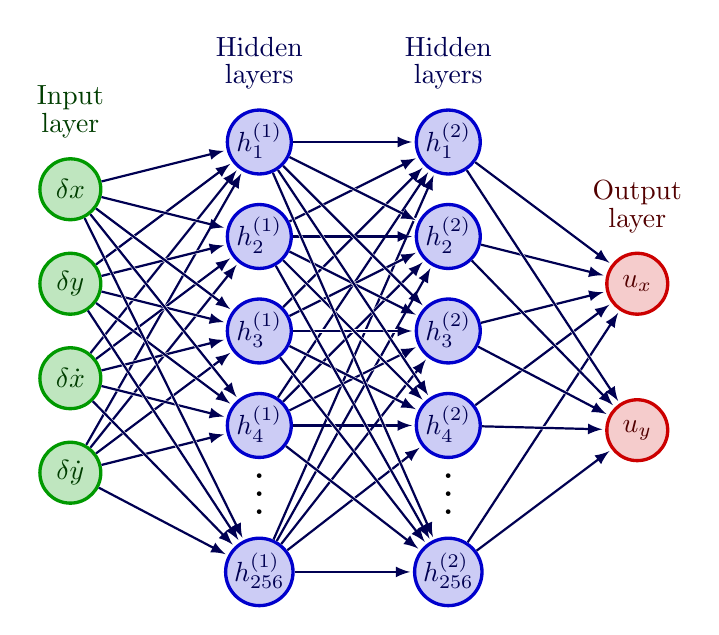
\begin{tikzpicture}[x=2.4cm,y=1.2cm]
	\readlist\Nnod{4,5,5,2} % array of number of nodes per layer
	\readlist\Nstr{n,256,k} % array of string number of nodes per layer
	\readlist\Cstr{x,h^{(\prev)},u} % array of coefficient symbol per layer
	\def\yshift{0.55} % shift last node for dots
	
	% LOOP over LAYERS
% LOOP over LAYERS
\foreachitem \N \in \Nnod{
  \def\lay{\Ncnt} % alias of index of current layer
  \pgfmathsetmacro\prev{int(\Ncnt-1)} % number of previous layer
  \foreach \i [evaluate={\c=int(\i==\N); 
  \layercheck=\ifnum\Ncnt=1 0 \else \ifnum\Ncnt=\Nnodlen 0 \else \yshift \fi \fi;
  \y=\N/2-\i-\c*\layercheck;
  \x=\lay; \n=\nstyle;
  \index=(\i<\N?int(\i):"\Nstr[\n]");}] in {1,...,\N}{ % loop over nodes
    % NODES
	\ifnum \lay=1
	\ifnum \i=1
		\node[node \n] (N\lay-\i) at (\x,\y) {$\delta x$};
	\fi
	\ifnum \i=2
		\node[node \n] (N\lay-\i) at (\x,\y) {$\delta y$};
	\fi
	\ifnum \i=3
		\node[node \n] (N\lay-\i) at (\x,\y) {$\delta {\dot{x}}$};
	\fi
	\ifnum \i=4
		\node[node \n] (N\lay-\i) at (\x,\y) {$\delta {\dot{y}}$};
	\fi
	\else \ifnum \lay=\Nnodlen
	\ifnum \i=1
		\node[node \n] (N\lay-\i) at (\x,\y) {$u_x$};
	\fi
	\ifnum \i=2
		\node[node \n] (N\lay-\i) at (\x,\y) {$u_y$};
	\fi
	\else
    \node[node \n] (N\lay-\i) at (\x,\y) {$\strut\Cstr[\n]_{\index}$};
    \fi \fi
    % CONNECTIONS
    \ifnumcomp{\lay}{>}{1}{ % connect to previous layer
      \foreach \j in {1,...,\Nnod[\prev]}{ % loop over nodes in previous layer
        \draw[white,line width=1.2,shorten >=1] (N\prev-\j) -- (N\lay-\i);
        \draw[connect] (N\prev-\j) -- (N\lay-\i);
      }
    %   \ifnum \lay=\Nnodlen
    %     \draw[connect] (N\lay-\i) --++ (0.5,0); % arrows out
    %   \fi
    }{
    %   \draw[connect] (0.5,\y) -- (N\lay-\i); % arrows in
    }
  }

  % Dots (skip first and last layers)
  \ifnum \lay>1 \ifnum \lay<\Nnodlen
    \path (N\lay-\N) --++ (0,1+\yshift) node[midway,scale=1.6] {$\vdots$}; % dots
  \fi \fi
}

  
	
	% LABELS
	\node[above=.1,align=center,mydarkgreen] at (N1-1.90) {Input\\[-0.2em]layer};
	\node[above=.1,align=center,mydarkblue] at (N2-1.90) {Hidden\\[-0.2em]layers};
	\node[above=.1,align=center,mydarkblue] at (N3-1.90) {Hidden\\[-0.2em]layers};
	\node[above=.1,align=center,mydarkred] at (N\Nnodlen-1.90) {Output\\[-0.2em]layer};
  \end{tikzpicture}
  \caption{Neural network architecture of the actor in the DDPG algorithm.}
\end{figure}
% \begin{figure}[H]
	\centering
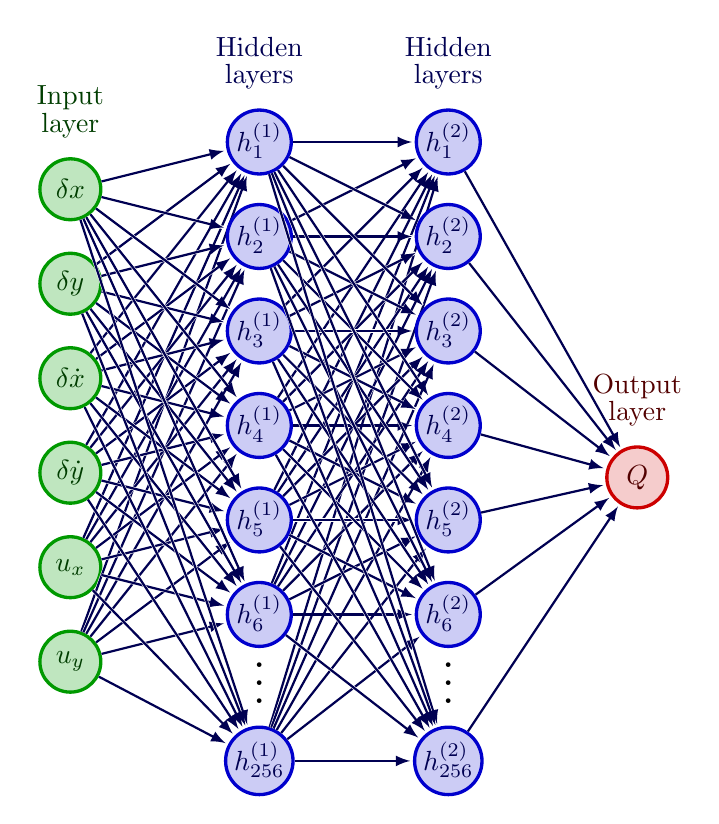
\begin{tikzpicture}[x=2.4cm,y=1.2cm]
	\readlist\Nnod{6,7,7,1} % array of number of nodes per layer
	\readlist\Nstr{n,256,k} % array of string number of nodes per layer
	\readlist\Cstr{x,h^{(\prev)},u} % array of coefficient symbol per layer
	\def\yshift{0.55} % shift last node for dots
	
	% LOOP over LAYERS
% LOOP over LAYERS
\foreachitem \N \in \Nnod{
  \def\lay{\Ncnt} % alias of index of current layer
  \pgfmathsetmacro\prev{int(\Ncnt-1)} % number of previous layer
  \foreach \i [evaluate={\c=int(\i==\N); 
  \layercheck=\ifnum\Ncnt=1 0 \else \ifnum\Ncnt=\Nnodlen 0 \else \yshift \fi \fi;
  \y=\N/2-\i-\c*\layercheck;
  \x=\lay; \n=\nstyle;
  \index=(\i<\N?int(\i):"\Nstr[\n]");}] in {1,...,\N}{ % loop over nodes
    % NODES
	\ifnum \lay=1
	\ifnum \i=1
		\node[node \n] (N\lay-\i) at (\x,\y) {$\delta x$};
	\fi
	\ifnum \i=2
		\node[node \n] (N\lay-\i) at (\x,\y) {$\delta y$};
	\fi
	\ifnum \i=3
		\node[node \n] (N\lay-\i) at (\x,\y) {$\delta {\dot{x}}$};
	\fi
	\ifnum \i=4
		\node[node \n] (N\lay-\i) at (\x,\y) {$\delta {\dot{y}}$};
	\fi
    \ifnum \i=5
        \node[node \n] (N\lay-\i) at (\x,\y) {$u_x$};
    \fi
    \ifnum \i=6
        \node[node \n] (N\lay-\i) at (\x,\y) {$u_y$};
    \fi
	\else \ifnum \lay=\Nnodlen
	\ifnum \i=1
		\node[node \n] (N\lay-\i) at (\x,\y) {$Q$};
	\fi
	\ifnum \i=2
		\node[node \n] (N\lay-\i) at (\x,\y) {$u_y$};
	\fi
	\else
    \node[node \n] (N\lay-\i) at (\x,\y) {$\strut\Cstr[\n]_{\index}$};
    \fi \fi
    % CONNECTIONS
    \ifnumcomp{\lay}{>}{1}{ % connect to previous layer
      \foreach \j in {1,...,\Nnod[\prev]}{ % loop over nodes in previous layer
        \draw[white,line width=1.2,shorten >=1] (N\prev-\j) -- (N\lay-\i);
        \draw[connect] (N\prev-\j) -- (N\lay-\i);
      }
    %   \ifnum \lay=\Nnodlen
    %     \draw[connect] (N\lay-\i) --++ (0.5,0); % arrows out
    %   \fi
    }{
    %   \draw[connect] (0.5,\y) -- (N\lay-\i); % arrows in
    }
  }

  % Dots (skip first and last layers)
  \ifnum \lay>1 \ifnum \lay<\Nnodlen
    \path (N\lay-\N) --++ (0,1+\yshift) node[midway,scale=1.6] {$\vdots$}; % dots
  \fi \fi
}

  
	
	% LABELS
	\node[above=.1,align=center,mydarkgreen] at (N1-1.90) {Input\\[-0.2em]layer};
	\node[above=.1,align=center,mydarkblue] at (N2-1.90) {Hidden\\[-0.2em]layers};
	\node[above=.1,align=center,mydarkblue] at (N3-1.90) {Hidden\\[-0.2em]layers};
	\node[above=.1,align=center,mydarkred] at (N\Nnodlen-1.90) {Output\\[-0.2em]layer};
  \end{tikzpicture}
  \caption{Neural network architecture of the critic in the DDPG algorithm.}
\end{figure}

\begin{figure}[!h]
    \begin{tikzpicture}
        \centering
        \hspace{-20pt}
            \begin{axis}[
                % xmode=log,
                % ymode=log,
                legend style={at={(1,1)},anchor=north east
                    ,draw=none,fill=none,inner sep=2mm},
                xlabel=X, % \hertz requires SIunits
                ylabel=Y,
                % title={Trajectory of the Spacecraft},
                % grid=both,
                % minor grid style={gray!25},
                % major grid style={gray!25},
                width=1\linewidth,
                enlarge y limits=0.25,
                no marks]
                \addplot[line width=1pt,solid,color=red] %
                table[x=x,y=y,col sep=comma]{plot_data/trajectory_latex.csv};
                \addlegendentry{Trajectory}
                \addplot[line width=1pt,dashed,color=black] %
                table[x=x,y=y,col sep=comma]{plot_data/state.csv};
                \addlegendentry{DDPG-DG Trajectory}
            \end{axis}
        \end{tikzpicture}
        \caption{Trajectory of the Spacecraft}
        \label{fig:trajectory}  
\end{figure}




\section{Training Validation}
The training of the guidance strategy is validated through a series of simulations that test the performance of the controller in various scenarios. The simulations involve transferring the spacecraft between Lyapunov orbits with different initial conditions and perturbations to evaluate the robustness and generalization capabilities of the guidance strategy. The training validation process demonstrates the effectiveness of the guidance strategy in handling complex mission scenarios and perturbations in the Earth-Moon system.	
\subsection{Perturbation Analysis}
The guidance strategy is evaluated under various perturbations to assess its robustness and resilience to disturbances. The perturbations include variations in the spacecraft's initial conditions, external disturbances, and model uncertainties. The guidance strategy is tested under different perturbation scenarios to evaluate its performance and stability in the presence of disturbances. The perturbation analysis provides insights into the controller's ability to adapt to changing conditions and maintain accurate trajectory following during the Lyapunov orbit transfer.
% \subsection{Generalization Across Missions}

\begin{figure}
\begin{tikzpicture}
	\hspace{-10pt}
	\begin{axis}
	  [
	  ytick={1,2},
	  yticklabels={DDPG DG, DDPG},
	  ]
	  \addplot+[
		boxplot prepared={
		  median=688.477151,
		  upper quartile=686.885704,
		  lower quartile=683.236397,
		  upper whisker=692.359664,
		  lower whisker=677.762436
		},
		] coordinates {};
	  \addplot+[
	  boxplot prepared={
		median=589.879372,
		upper quartile=690.021882,
		lower quartile=299.609773,
		upper whisker=692.640044,
		lower whisker=286.00839
	  },
	  ] coordinates {};
	\end{axis}
	% disturbance usingg 1000 samples mont carlo
  \end{tikzpicture}
  \caption{
	Comparison of the total rewards obtained by the DDPG and DDPG DG algorithms in the presence of disturbances.
}
\end{figure}







\begin{figure}
	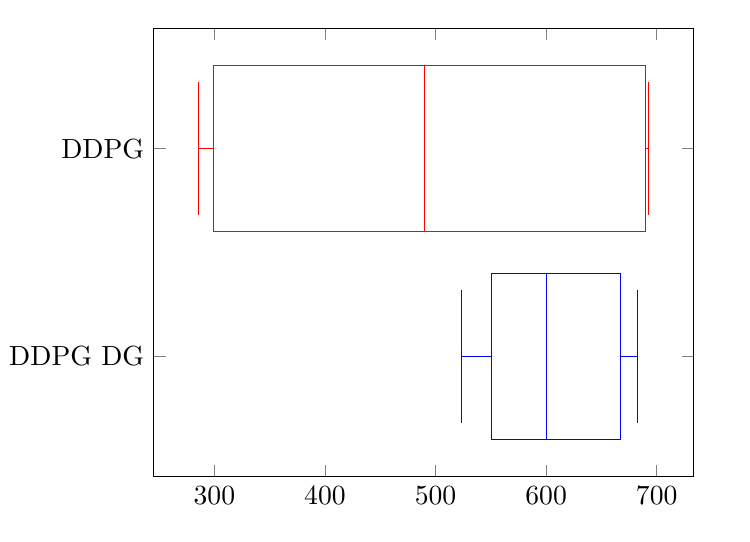
\begin{tikzpicture}
		\hspace{-10pt}
		\begin{axis}
		  [
		  ytick={1,2},
		  yticklabels={DDPG DG, DDPG},
		  ]
		  \addplot+[
			boxplot prepared={
  lower whisker=523.236397,
  lower quartile=550.762436,
  median=600.477151,
  upper quartile=666.885704,
  upper whisker=682.359664
},
			] coordinates {};
		  \addplot+[
			boxplot prepared={
				lower whisker=286.00839,
				lower quartile=299.609773,
				median=489.879372,
				upper quartile=690.021882,
				upper whisker=692.640044
			  },
		  ] coordinates {};
		\end{axis}
		% non ideal thrust engine using 1000 samples mont carlo
	  \end{tikzpicture}
	  \caption{
		Comparison of the total rewards obtained by the DDPG and DDPG DG algorithms in the presence of non-ideal thrust engine models.
	}
\end{figure}

\begin{figure}
	\begin{tikzpicture}
		\hspace{-10pt}
		\begin{axis}
		  [
		  ytick={1,2},
		  yticklabels={DDPG DG, DDPG},
		  ]
		  \addplot+[
boxplot prepared={
	lower whisker=681.515208,
	lower quartile=684.773397,
	median=686.437301,
	upper quartile=686.945523,
	upper whisker=690.203711
  },
			] coordinates {};
		  \addplot+[
			boxplot prepared={
  lower whisker=286.00839,
  lower quartile=299.609773,
  median=689.879372,
  upper quartile=690.021882,
  upper whisker=689.640044
},
		  ] coordinates {};
		\end{axis}
		% model parameter variation 1000 samples mont carlo
	  \end{tikzpicture}
	  \caption{
		Comparison of the total rewards obtained by the DDPG and DDPG DG algorithms in the presence of model parameter variations.
	}
\end{figure}









\section{Real-Time Implementation}
The guidance strategy is implemented in real-time using a software-in-the-loop (SIL) simulation environment to validate its performance and computational efficiency. The real-time implementation involves running the guidance strategy on a high-fidelity simulation model of the CR3BP with low-thrust terms and evaluating its performance in real-world scenarios. The real-time implementation demonstrates the feasibility of deploying the guidance strategy on an actual spacecraft and its ability to handle the computational requirements of autonomous navigation in deep-space missions.
\subsection{ROS-Based System Integration}
The guidance strategy is integrated into a Robot Operating System (ROS) framework to facilitate communication between the guidance controller and the spacecraft's onboard systems. The ROS-based system integration enables seamless data exchange between the guidance strategy, the spacecraft's sensors, and the low-thrust propulsion system. The integration of the guidance strategy with ROS enhances the autonomy and adaptability of the spacecraft's navigation system, enabling it to respond to changing mission requirements and environmental conditions.
\subsection{Computational Efficiency in Real-Time Execution}
The computational efficiency of the guidance strategy is evaluated in real-time execution to ensure that it meets the stringent timing requirements of deep-space missions. The guidance strategy is benchmarked against the mission's timing constraints to verify that it can generate control commands within the specified time frame. The computational efficiency analysis ensures that the guidance strategy can operate in real-time on a spacecraft's onboard computer system and meet the mission's performance requirements.
\section{Conclusion}
The proposed guidance framework leverages reinforcement learning to develop a robust differential game-based guidance strategy for low-thrust spacecraft in multi-body dynamical environments. The guidance strategy is designed to handle large initial deviations, enhance resilience against disturbances, and augment conventional targeting guidance methods. The framework is implemented using the Deep Deterministic Policy Gradient (DDPG) algorithm, which is a model-free, off-policy reinforcement learning algorithm that combines the stability of deterministic policy gradients with the flexibility of deep neural networks. The guidance strategy is trained using a differential game formulation, where two spacecraft are modeled as agents in a competitive game. The agents interact with each other and the environment to learn optimal control policies that maximize their rewards. The guidance strategy is implemented in a simulated environment that captures the dynamics of the Circular Restricted Three-Body Problem (CR3BP) with low-thrust terms. The effectiveness of the guidance strategy is demonstrated through sample transfers between Lyapunov orbits in the Earth-Moon system, where the controller exhibits strong robustness to perturbations and generalizes effectively across different mission scenarios and low-thrust engine models. The proposed guidance framework represents a significant advancement in autonomous spacecraft navigation in complex gravitational environments and has the potential to enable a wide range of deep-space missions.








% \begin{table}[htbp]
% \caption{Table Type Styles}
% \begin{center}
% \begin{tabular}{|c|c|c|c|}
% \hline
% \textbf{Table}&\multicolumn{3}{|c|}{\textbf{Table Column Head}} \\
% \cline{2-4}
% \textbf{Head} & \textbf{\textit{Table column subhead}}& \textbf{\textit{Subhead}}& \textbf{\textit{Subhead}} \\
% \hline
% copy& More table copy$^{\mathrm{a}}$& &  \\
% \hline
% \multicolumn{4}{l}{$^{\mathrm{a}}$Sample of a Table footnote.}
% \end{tabular}
% \label{tab1}
% \end{center}
% \end{table}

% \begin{figure}[htbp]
% \centerline{\includegraphics{fig1.png}}
% \caption{Example of a figure caption.}
% \label{fig}
% \end{figure}




% \section*{References}


\begin{thebibliography}{00}
\bibitem{Sutton} Sutton, R. S., Barto, A. G. (2018 ). Reinforcement Learning: An Introduction. The MIT Press.
% \bibitem{b2} J. Clerk Maxwell, A Treatise on Electricity and Magnetism, 3rd ed., vol. 2. Oxford: Clarendon, 1892, pp.68--73.
% \bibitem{b3} I. S. Jacobs and C. P. Bean, ``Fine particles, thin films and exchange anisotropy,'' in Magnetism, vol. III, G. T. Rado and H. Suhl, Eds. New York: Academic, 1963, pp. 271--350.
% \bibitem{b4} K. Elissa, ``Title of paper if known,'' unpublished.
% \bibitem{b5} R. Nicole, ``Title of paper with only first word capitalized,'' J. Name Stand. Abbrev., in press.
% \bibitem{b6} Y. Yorozu, M. Hirano, K. Oka, and Y. Tagawa, ``Electron spectroscopy studies on magneto-optical media and plastic substrate interface,'' IEEE Transl. J. Magn. Japan, vol. 2, pp. 740--741, August 1987 [Digests 9th Annual Conf. Magnetics Japan, p. 301, 1982].
% \bibitem{b7} M. Young, The Technical Writer's Handbook. Mill Valley, CA: University Science, 1989.
% \bibitem{b8} D. P. Kingma and M. Welling, ``Auto-encoding variational Bayes,'' 2013, arXiv:1312.6114. [Online]. Available: https://arxiv.org/abs/1312.6114
% \bibitem{b9} S. Liu, ``Wi-Fi Energy Detection Testbed (12MTC),'' 2023, gitHub repository. [Online]. Available: https://github.com/liustone99/Wi-Fi-Energy-Detection-Testbed-12MTC
% \bibitem{b10} ``Treatment episode data set: discharges (TEDS-D): concatenated, 2006 to 2009.'' U.S. Department of Health and Human Services, Substance Abuse and Mental Health Services Administration, Office of Applied Studies, August, 2013, DOI:10.3886/ICPSR30122.v2
% \bibitem{b11} K. Eves and J. Valasek, ``Adaptive control for singularly perturbed systems examples,'' Code Ocean, Aug. 2023. [Online]. Available: https://codeocean.com/capsule/4989235/tree
\end{thebibliography}

% \vspace{12pt}
% \color{red}
% IEEE conference templates contain guidance text for composing and formatting conference papers. Please ensure that all template text is removed from your conference paper prior to submission to the conference. Failure to remove the template text from your paper may result in your paper not being published.

\end{document}
